\documentclass[10pt]{article}
\usepackage[polish]{babel}
\usepackage[utf8]{inputenc}
\usepackage[T1]{fontenc}
\usepackage{amsmath}
\usepackage{amsfonts}
\usepackage{amssymb}
\usepackage[version=4]{mhchem}
\usepackage{stmaryrd}
\usepackage{graphicx}
\usepackage[export]{adjustbox}
\graphicspath{ {./images/} }

\title{POLITECHNIKA \\
 GDAŃSKA }

\author{}
\date{}


\begin{document}
\maketitle
\section*{CENTRUM MATEMATYKI}
\section*{OD SZKOLNIAKA DO ŻAKA}
\section*{klasy 7 i 8 szkoły podstawowej}
rok szkolny 2021/2022

\section*{Zadania - etap III}
Zadanie 1. W trapezie równoramiennym przekątne o długości 14 przecinają się w stosunku 3:4 i tworzą z podstawami kąty o mierze \(60^{\circ}\). Oblicz pole i obwód tego trapezu.

Zadanie 2. Wykaż, że suma pól „półksiężyców" przedstawionych na rysunku jest równa polu kwadratu ABCD.\\
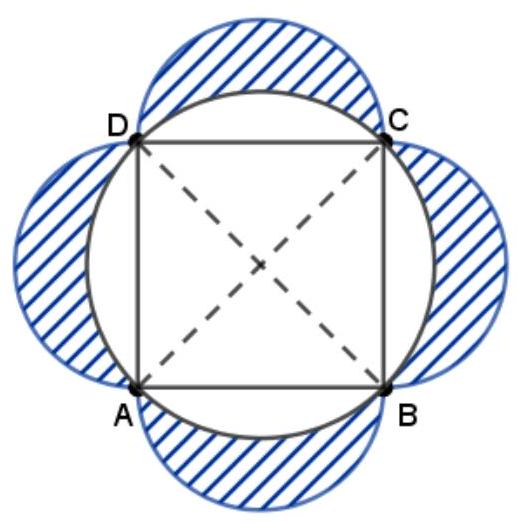
\includegraphics[max width=\textwidth, center]{2024_11_21_dd87acbd3841c21f8f46g-1}

Zadanie 3. Janek przejechał na rowerze odległość 20 km , a z powrotem przeszedł tą samą trasę pieszo z prędkością 3 razy mniejszą. Ile wynosiła prędkość jazdy a ile prędkość marszu, jeśli cała podróż trwała 5 godzin i 20 minut?

Zadanie 4. Wyznacz liczby naturalne \(a\) i \(b\), jeżeli wiadomo, że \(N W D(a, b)=6\) i \(N W W(a, b)=36\).

Zadanie 5. Znajdź cztery najmniejsze kolejne liczby naturalne nieparzyste, których suma jest podzielna przez 10. Zapisz wszystkie obliczenia.


\end{document}